%----------------------------------------------------------------------------------------
%	PACKAGES AND THEMES
%----------------------------------------------------------------------------------------
\documentclass[aspectratio=169,xcolor=dvipsnames]{beamer}
\usetheme{Simple}
\usepackage{amsfonts, amssymb, amsmath}
\usepackage{caption}
\usepackage{subcaption}
\usepackage{hyperref} % link crossrefs and toc
\hypersetup{
    colorlinks=true,
    linkcolor=cyan,
    filecolor=magenta,
    urlcolor=cyan,
    citecolor=black
}
\usepackage{pdfpages}
\usepackage{graphicx} % Allows including images
\graphicspath{{../../img}}
\usepackage{booktabs} % Allows the use of \toprule, \midrule and \bottomrule in tables
\usepackage{siunitx}
\renewcommand{\inserttotalframenumber}{\pageref{lastslide}}

%----------------------------------------------------------------------------------------
%	TITLE PAGE
%----------------------------------------------------------------------------------------

% The title
\title{Real-time Posture Tracking using Gyroscope}
\subtitle{Internet of Things Project}
\vspace{10cm}
\author[Pin-Yen]{Pratyusha R - C Ramprakash - Skanda Prasad}
\institute % Your institution may be shorthand to save space
{
    % Your institution for the title page
    Department of Electronics and Communication Engineering

    6th Semester, A Section
    \vskip 3pt
}
\date{June 24, 2021} % Date, can be changed to a custom date


%----------------------------------------------------------------------------------------
%	PRESENTATION SLIDES
%----------------------------------------------------------------------------------------

\begin{document}

\begin{frame}
    % Print the title page as the first slide
    \begin{figure}
     \centering
     \begin{subfigure}[b]{0.49\textwidth}
         \centering
         
\includegraphics[scale=0.35]{ecelogo.png}
     \end{subfigure}
     \hfill
     \begin{subfigure}[b]{0.49\textwidth}
         \centering
         
\includegraphics[scale=0.35]{New_NIE_Logo.png}
     \end{subfigure}
     \end{figure}
    \titlepage
\end{frame}
%---------------------------------------------------

\begin{frame}{Overview}
    \tableofcontents
\end{frame}

%------------------------------------------------
\section{Introduction}
%------------------------------------------------

\begin{frame}{Introduction}
        \vspace{0.5cm}
        \begin{itemize}
        \item Bad habits such as slouching cause muscle fatigue and tension
            that ultimately lead to poor posture.
        \item Slouching can cause the spinal ligaments to stretch beyond their
            healthy limit, and poor posture can strain your spinal discs.
        \item To correct bad posture it is crucial to monitor posture.
        \item \textit{``If you can’t measure it, you can’t improve it.''}
            –\textit{ Peter Drucker}
    \end{itemize}
    \hfill
     \begin{figure}
        \centering
        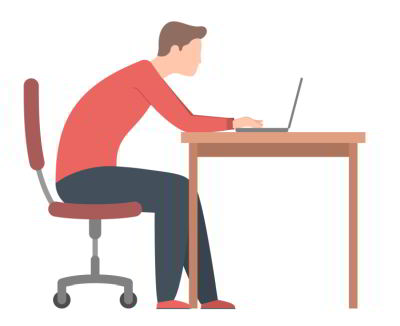
\includegraphics[scale=0.25]{slouching_bad_posture.jpg}
        \caption{Slouching posture}
        \label{fig:good}
    \end{figure}
\end{frame}

%------------------------------------------------
\section{Data Collection}

\begin{frame}{Collection of Data}
    \begin{itemize}
        \item Espressif's ESP8266 NodeMCU was used to interface the MPU6050
            Gyro-Accelerometer by employing I\textsuperscript{2}C Serial Communication Protocol.
        \item It was programmed to generate the data representing rotational
            change in all the three axes.
        \item Trials were conducted to determine how the data changes in
            real-time with respect to movement of body.
    \end{itemize}

\end{frame}

%---------------------------------------------------------
\begin{frame}{Rule Based Posture Detection}
    Analysing Data:
   \begin{figure}
       \centering
       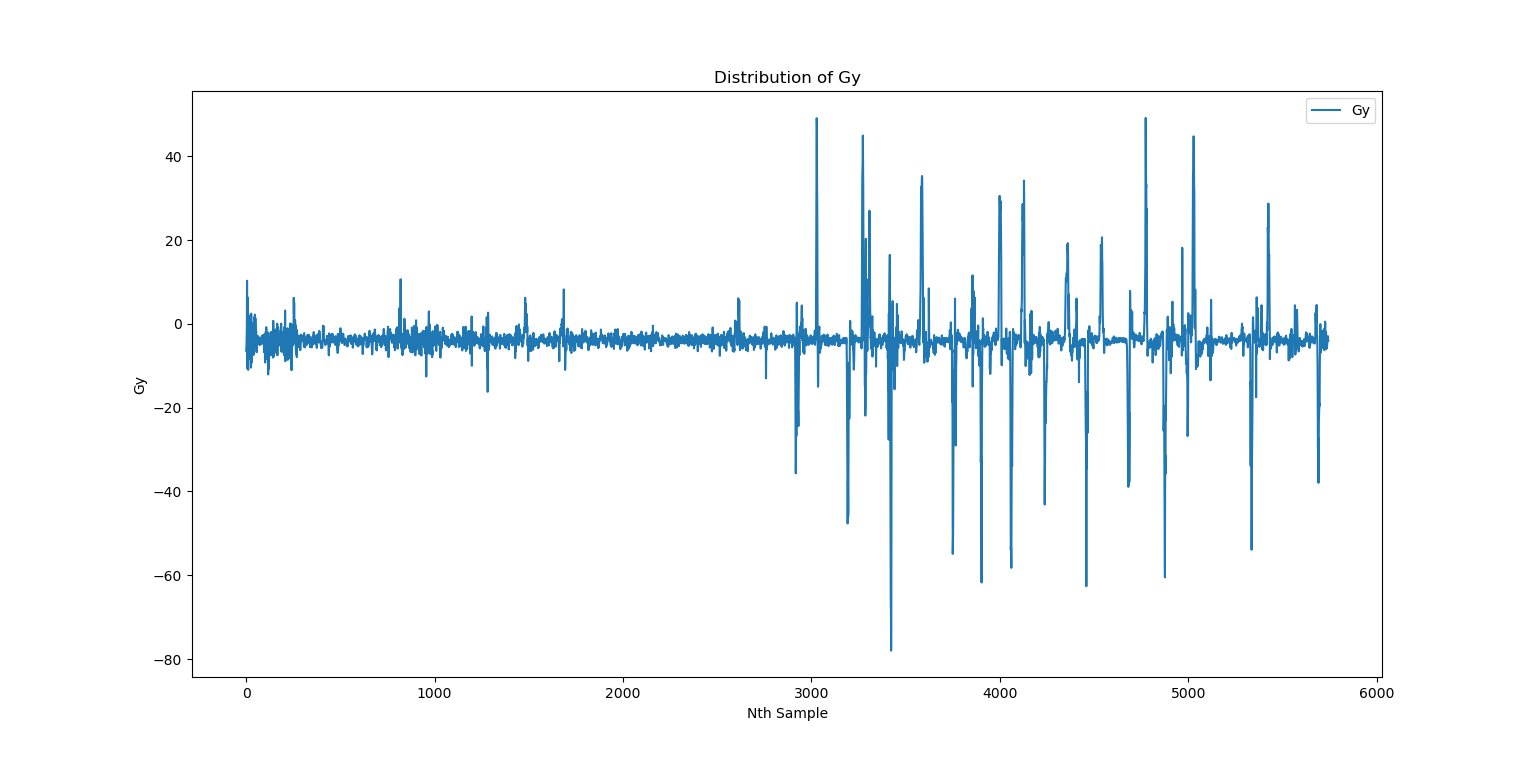
\includegraphics[scale=0.3]{gy_dist.png}
       \caption{Depicting Collected Data of Gy}
       \label{fig:piximage}
   \end{figure}
  \end{frame}

%-----------------------------------------------------------
\begin{frame}{Rule Based Posture Detection}
    \begin{itemize}
        \item We are considering the $Gy$ axis as when the subject slouches
            there is motion only in the Y-axis.
        \item We observe that every time the subject
            \begin{itemize}
                \item Slouches $-$ Negative spike in the $Gy$ value.
                \item Comes back to a good posture $-$ Positive spike in the
                    $Gy$ value.
            \end{itemize}
        \item Mapping \qty{\pm15}{\degree\per\second} as thresholds for positive and negative
            spikes respectively.
        \item Then return the time spent in each posture in seconds.
    \end{itemize}
\end{frame}

%-----------------------------------------------------------



%-----------------------------------------------------------
\section{Proposed Method}

\begin{frame}{Proposed Method}

 \begin{columns}[c]
  \column{.4\textwidth}
    \begin{itemize}
        \item Collect the gyroscope data using MPU6050.
        \item Process it with Microprocessor Unit and send it to a host system,
            which sends HTTP \texttt{POST} requests to update a Google Sheet.
        \item To store data we are using Goggle Sheets as our database.
        \item Then the web application sends HTTP \texttt{GET} requests using
            Google Sheets API.
        \item We display the results using a simple dashboard.
    \end{itemize}
    \column{.4\textwidth}
    \begin{figure}
        \centering
            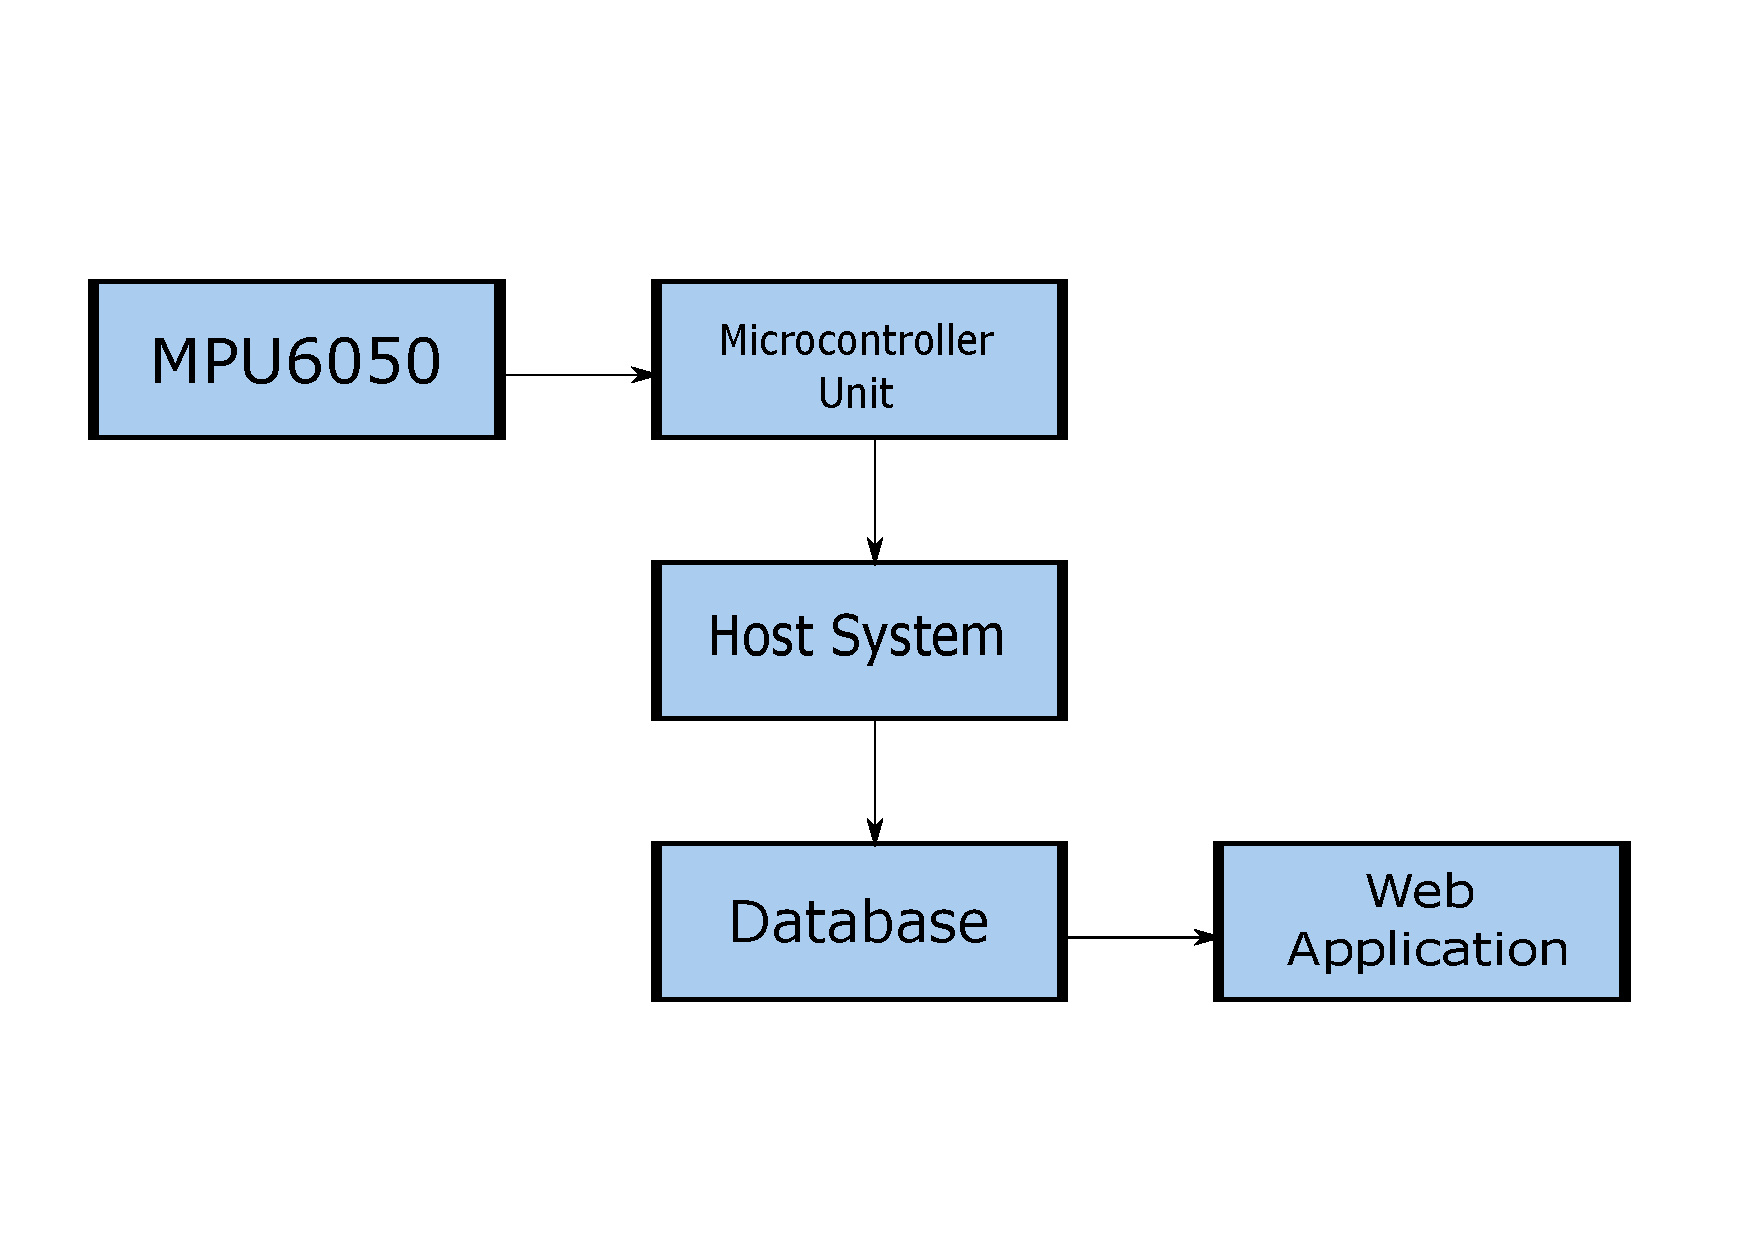
\includegraphics[scale=0.2]{flowchart.pdf}
            \caption{Depicting Collected Data of Gy}
            \label{fig:archi}
        \end{figure}
     \end{columns}
\end{frame}

%------------------------------------------------

\begin{frame}{Obtained Results}
    \begin{figure}
        \centering
        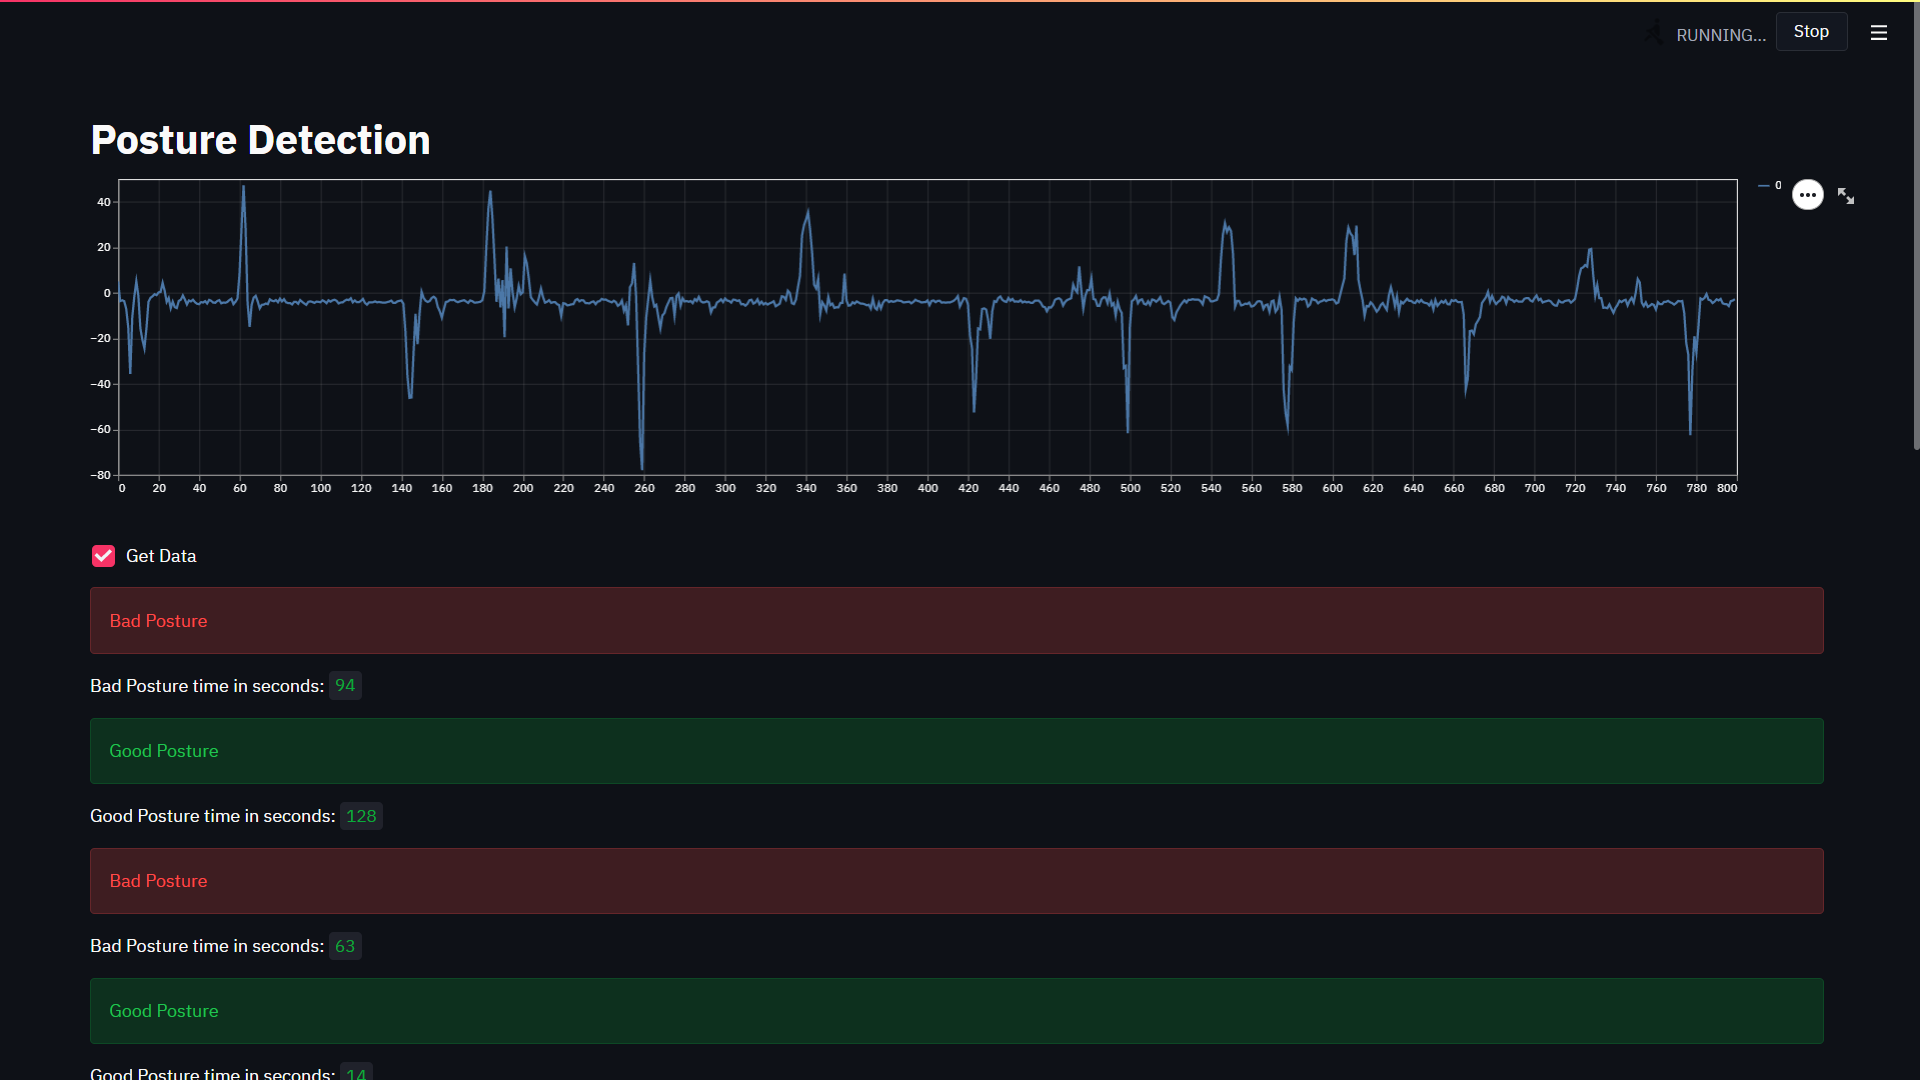
\includegraphics[scale=0.18]{webappss2.png}
        \caption{Plotting data and showing posture changes in real-time}
        \label{fig:results}
    \end{figure}

\end{frame}
%-----------------------------------------------

%------------------------------------------------
\section{Conclusions and Future Work}
%------------------------------------------------

\begin{frame}{Conclusions and Future Work}
    \begin{block}{Outcomes}
        \begin{itemize}
            \item Simplicity
            \item Cost-effectiveness
        \end{itemize}
    \end{block}
    \begin{block}{Limitations}
        \begin{itemize}
            \item Can be susceptible to ``noisy'' movements.
            \item Google Sheets is not a good long-term choice
        \end{itemize}
    \end{block}
    \begin{block}{Future Work}
        \begin{itemize}
            \item Be able to detect more range of activities.
            \item Send HTTP requests without the intervention of host system.
            \item Give a detailed analysis of their posture and predict it's
                effect on health.
        \end{itemize}

    \end{block}
\end{frame}

%-----------------------------------------------
\begin{frame}
     \Huge{\centerline{Questions}}
     \vspace{1cm}
    {\large \centerline{GitHub: \url{https://github.com/skandaprasad/mpu6050-datalogger}}}
\end{frame}
\end{document}
